% (C) Savoir-faire Linux, 2017 
% authored by Marc Lijour, March 2017 
% Some art belong to their respective authors, as indicated in the document
% 
% ======================================================================================================
%                                     FINTECH
% ======================================================================================================
\section{Insights on FinTech}
\frame{
	\begin{block}{}
		\begin{quote}
			{\Huge 20\% of the world's economy will be digital by 2020.} \\
			\vspace{1em}
			\hfill ---Accenture \#techvision2016
		\end{quote}
	\end{block}
}

\frame{
	\frametitle{FinTech: Technology resets the game for FSIs}
	\begin{itemize}
		\item ``Silicon Valley is coming'' ---Jamie Dimon, CEO, JP Morgan Chase
		\pause
		\item ``Half of the world's banks will disappear'' --- Francisco Gonzalez, Chief Executive, BBVA \vspace{2em}
		\pause
		\item Bitcoin $\rightarrow$ almost free remittances, cashless society?
		\pause
		\item Lending Club $\rightarrow$ individual to individual, shortcircuiting the bank
		\pause
		\item Wealthsimple $\rightarrow$ intelligent investment, Bye bye management fees
		\pause
		\item Square, Venmo $\rightarrow$ payment on the go
		\item etc
	\end{itemize}
}

\frame{
	\frametitle{The Milenials}
	\begin{figure} % https://www.flickr.com/photos/statefarm/26663820390
		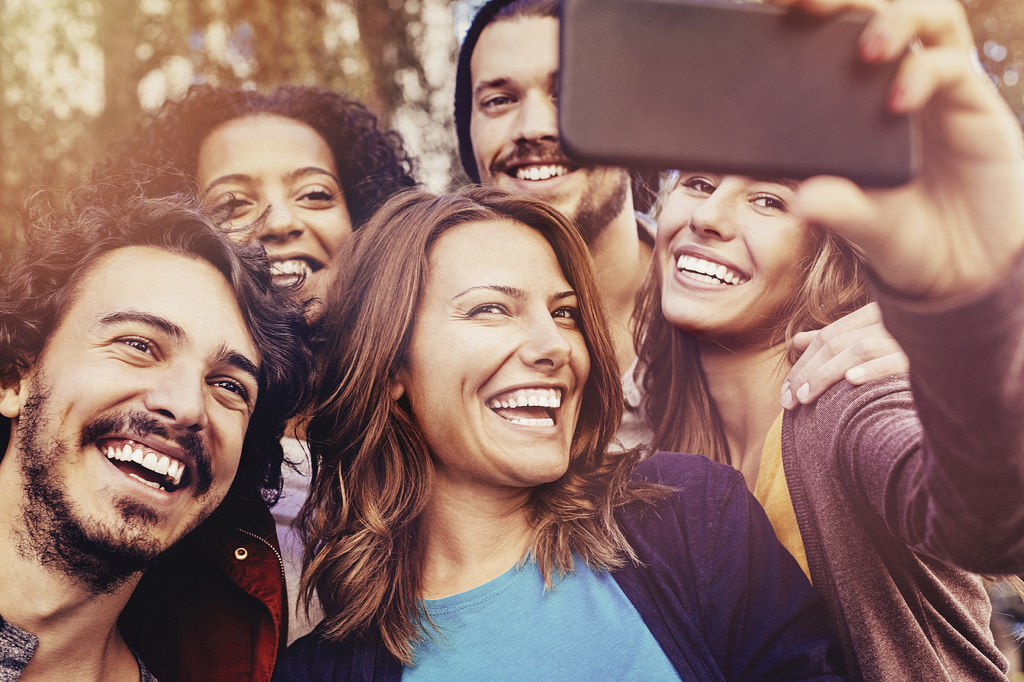
\includegraphics[width=11cm]{../pics/statefarm-milenials-CC-BY}
	\end{figure}
	\tiny \copyright \href{https://www.flickr.com/photos/statefarm/26663820390}{State Farm} (CC-BY license)
}

\begin{frame}
	\frametitle{Open Source runs (almost) Everything}
	\framesubtitle{2015 was an inflexion point}
	\begin{figure} % extracts from articles and other sources published on the Web
		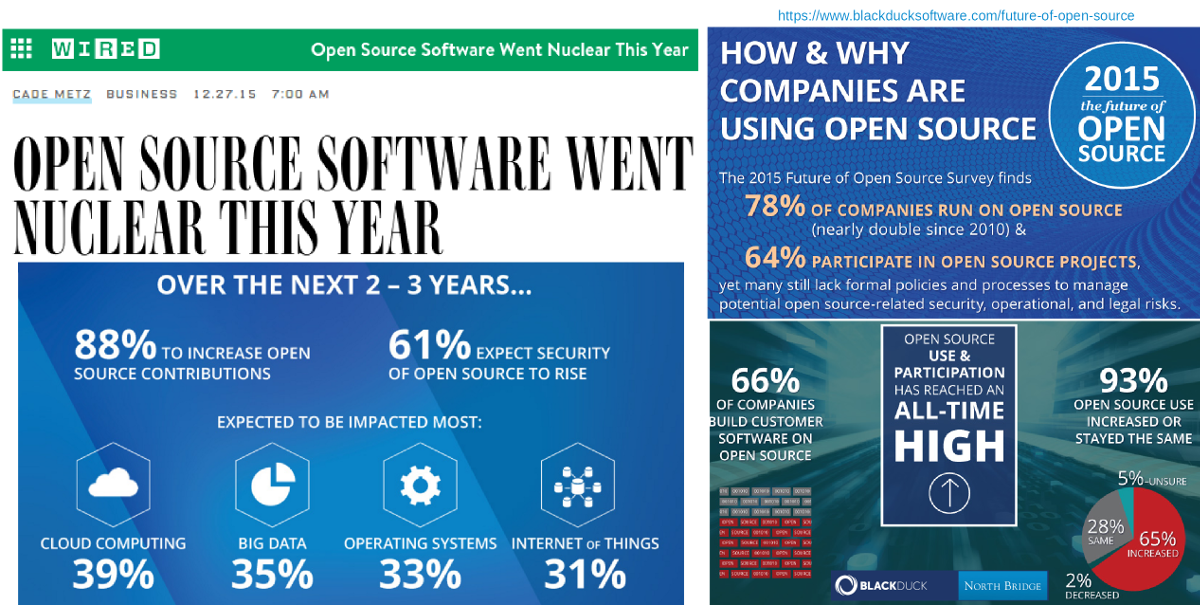
\includegraphics[width=11cm]{../pics/pic-open-source-went-nuclear-non-interlaced}
	\end{figure}
\end{frame}

\frame{
	\frametitle{A threatening Gap for Incubants}
	\begin{columns}[t]
		\column{0.5\textwidth}
		{\center Start ups}
		\begin{itemize}
			\item Small
			\item Agile
			\item Open Source
			\item Bootstrapping
		\end{itemize}
		
		\column{0.5\textwidth}
		{\center Old Bank} 
		\begin{itemize}
			\item Very large (often dealing with multiple jurisdictions)
			\item Siloed and burdened with processes
			\item Legacy technology (mainframe, COBOL, etc)
			\item Supporting a branch network (brick and mortar)
		\end{itemize}
		
	\end{columns}
}

\frame{
	\frametitle{Areas of Focus for Financial Services Institutions (FSIs)}
	\begin{columns}
		\column{0.3\textwidth}\center
		\begin{figure}
			
\includegraphics[width=1.5cm]{../pics/icons/headphones-8x}
		\end{figure}
		\tiny Reduce Customer Friction

		\column{0.3\textwidth}\center
		\begin{figure}
			
\includegraphics[width=1.5cm]{../pics/icons/droplet-8x}
		\end{figure}
		\tiny Save on Costs

		\column{0.3\textwidth}\center
		\begin{figure}
			
\includegraphics[width=1.5cm]{../pics/icons/graph-8x}
		\end{figure}
		\tiny Generate New Revenues

	\end{columns}
}

\frame{
	\frametitle{Technology Tsunami in Progress}
	\framesubtitle{\ldots and as many job opportunities\ldots}
	\begin{itemize}
		\item DevOps $\rightarrow$ BizDevOps
		\pause
		\item Blockchain 
		\pause
		\item Big Data and Analytics (Hadoop is hot)
		\pause
		\item Artificial Intelligence, Machine Learning 
	\end{itemize}
}

\frame{
	\frametitle{The Challenge for FSIs}
	\begin{block}{}
		\begin{quote}
			{\Huge To generate relevant and valuable services for the customer, as expectations rise, \\
			and to do it fast enough.} \\
		\end{quote}
	\end{block}
}

